\documentclass{article}%
\usepackage[T1]{fontenc}%
\usepackage[utf8]{inputenc}%
\usepackage{lmodern}%
\usepackage{textcomp}%
\usepackage{lastpage}%
\usepackage{geometry}%
\geometry{margin=0.2in}%
\usepackage{graphicx}%
%
\title{Report on AustraliaWeather dataset}%
\author{Classify2TeX}%
\usepackage{amsmath}%
\usepackage{amssymb}%
\usepackage{enumitem}%
%
\begin{document}%
\normalsize%
\maketitle%
\newpage%
\tableofcontents%
\newpage%
\section{Exploratory Data Analysis}%
\label{sec:ExploratoryDataAnalysis}%
\subsection{Non{-}Null Count, Dtype of features}%
\label{subsec:Non{-}NullCount,Dtypeoffeatures}%
The table 1 provides information about the dataset, including the number of non-null values and the data types of each feature.%


\begin{table}[h!]%
\caption{Dataset Columns Information}%
\vspace{0.2cm}%
\centering%
\begin{tabular}{|c||c||c||c|}%
\hline%
Index&Column&Non{-}Null Count&Dtype\\%
\hline%
0&Date&3000&object\\%
1&Location&3000&object\\%
2&MinTemp&2961&float64\\%
3&MaxTemp&2970&float64\\%
4&Rainfall&2922&float64\\%
5&Evaporation&1667&float64\\%
6&Sunshine&1506&float64\\%
7&WindGustDir&2791&object\\%
8&WindGustSpeed&2793&float64\\%
9&WindDir9am&2787&object\\%
10&WindDir3pm&2915&object\\%
11&WindSpeed9am&2966&float64\\%
12&WindSpeed3pm&2937&float64\\%
13&Humidity9am&2939&float64\\%
14&Humidity3pm&2898&float64\\%
15&Pressure9am&2681&float64\\%
16&Pressure3pm&2684&float64\\%
17&Cloud9am&1832&float64\\%
18&Cloud3pm&1771&float64\\%
19&Temp9am&2958&float64\\%
20&Temp3pm&2918&float64\\%
21&RainToday&2922&object\\%
22&RainTomorrow&2926&object\\%
\hline%
\end{tabular}%
\end{table}

%
\newpage%
\subsection{Descriptive Statistics}%
\label{subsec:DescriptiveStatistics}%
The table 2 provides descriptive statistics for the dataset, including the count, mean, standard deviation, minimum, and maximum values.%


\begin{table}[h!]%
\caption{Dataset Descriptive Statistics}%
\vspace{0.2cm}%
\centering%
\begin{tabular}{|c||c||c||c||c||c||c||c||c||c|}%
\hline%
Index&Column Name/Statistic&count&mean&std&min&25\%&50\%&75\%&max\\%
\hline%
0&MinTemp&2961.0&11.96&6.33&{-}5.0&7.5&11.8&16.8&29.4\\%
1&MaxTemp&2970.0&22.97&7.17&{-}1.9&17.6&22.3&28.1&46.1\\%
2&Rainfall&2922.0&2.15&7.79&0.0&0.0&0.0&0.8&225.0\\%
3&Evaporation&1667.0&5.35&3.75&0.0&2.6&4.6&7.4&31.0\\%
4&Sunshine&1506.0&7.46&3.87&0.0&4.6&8.2&10.7&14.5\\%
5&WindGustSpeed&2793.0&39.81&13.33&9.0&31.0&39.0&46.0&106.0\\%
6&WindSpeed9am&2966.0&14.02&8.93&0.0&7.0&13.0&19.0&65.0\\%
7&WindSpeed3pm&2937.0&18.66&8.87&0.0&13.0&19.0&24.0&65.0\\%
8&Humidity9am&2939.0&69.13&18.85&4.0&57.0&70.0&83.0&100.0\\%
9&Humidity3pm&2898.0&51.86&20.79&4.0&37.0&52.0&66.0&100.0\\%
10&Pressure9am&2681.0&1017.89&7.12&982.2&1013.2&1017.8&1022.6&1040.3\\%
11&Pressure3pm&2684.0&1015.52&7.08&984.2&1010.6&1015.5&1020.3&1037.6\\%
12&Cloud9am&1832.0&4.49&2.88&0.0&1.0&5.0&7.0&8.0\\%
13&Cloud3pm&1771.0&4.58&2.72&0.0&2.0&5.0&7.0&8.0\\%
14&Temp9am&2958.0&16.74&6.44&{-}4.1&12.0&16.25&21.4&35.2\\%
15&Temp3pm&2918.0&21.43&6.99&{-}1.0&16.23&20.7&26.3&44.5\\%
\hline%
\end{tabular}%
\end{table}

%
\newpage%
\subsection{Distribution of features}%
\label{subsec:Distributionoffeatures}%
This section provides a visual representation of the distribution of features in the dataset using histograms (numerical features) and bar charts (categorical features). These visualizations can help in understanding the data.%
\subsubsection{Histograms of Numerical columns}%
\label{ssubsec:HistogramsofNumericalcolumns}%
The histograms below show the distribution of numerical features in the dataset.%


\begin{figure}[h!]%
\centering%
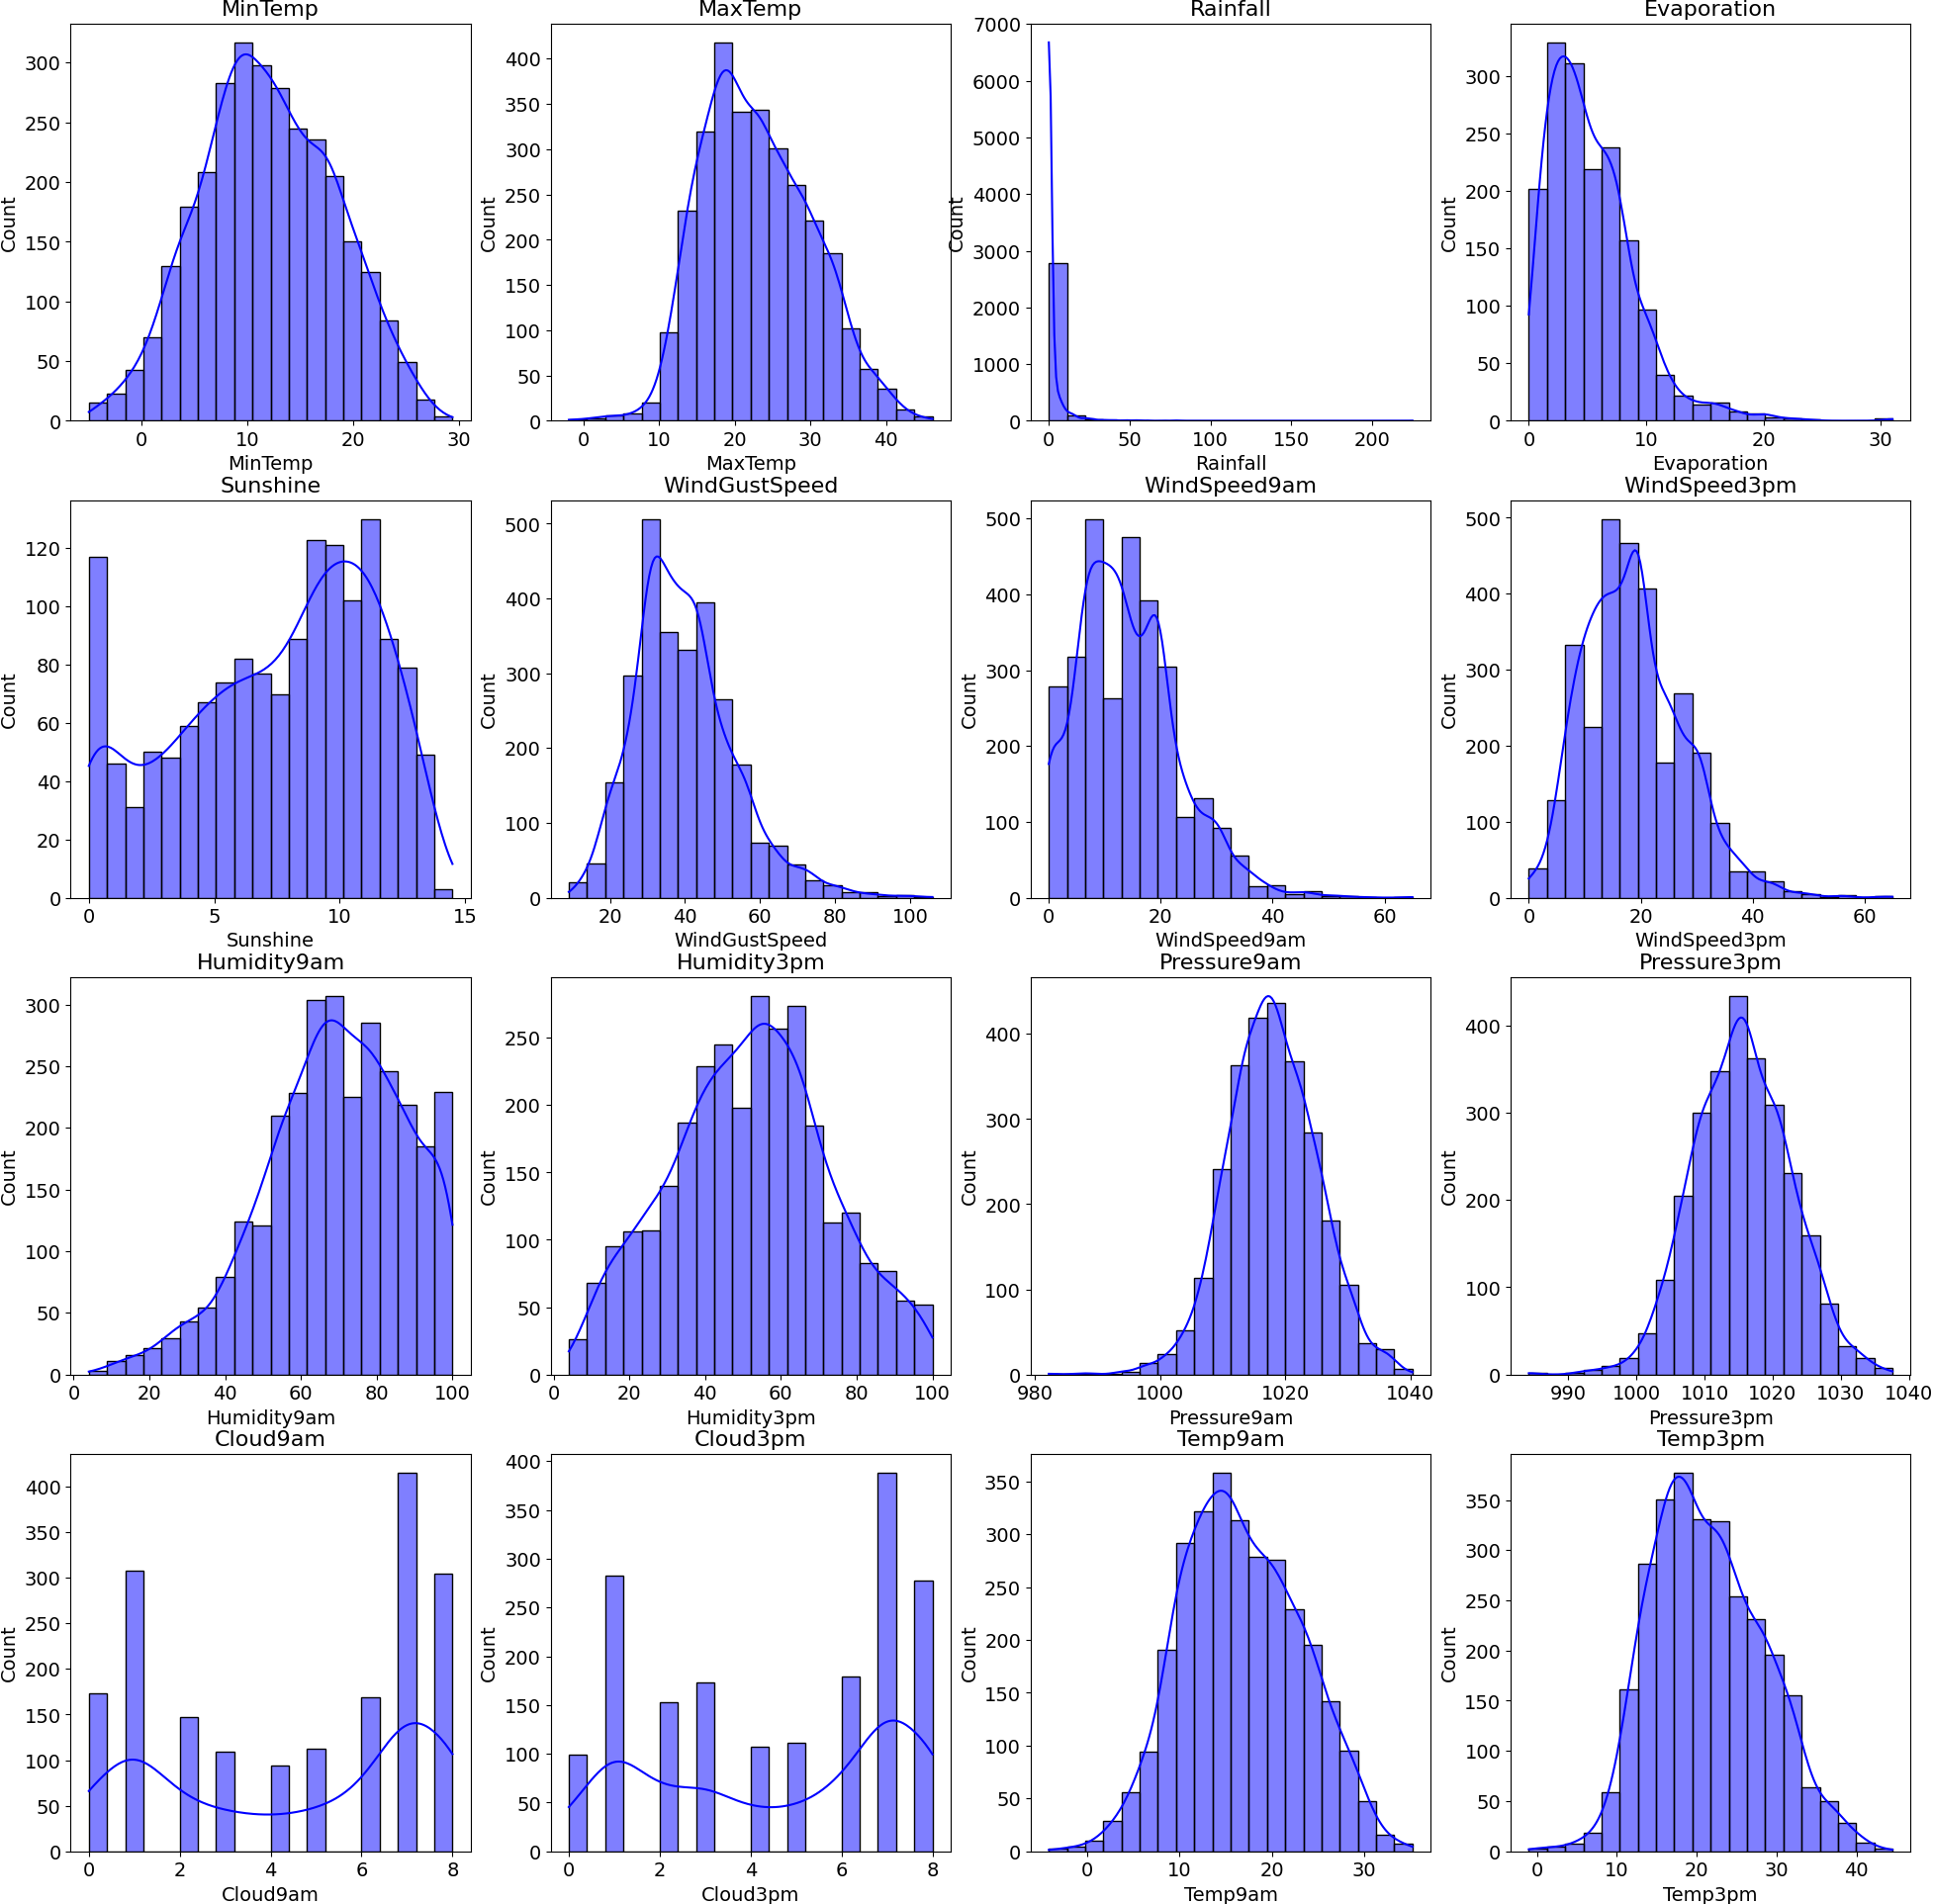
\includegraphics[width=460px]{EDA/histograms.png}%
\caption{Histograms of Numerical columns}%
\end{figure}

%
\newpage%
\subsubsection{Bar Charts of Categorical columns}%
\label{ssubsec:BarChartsofCategoricalcolumns}%
The bar charts below show the distribution of categorical features in the dataset.%


\begin{figure}[h!]%
\centering%
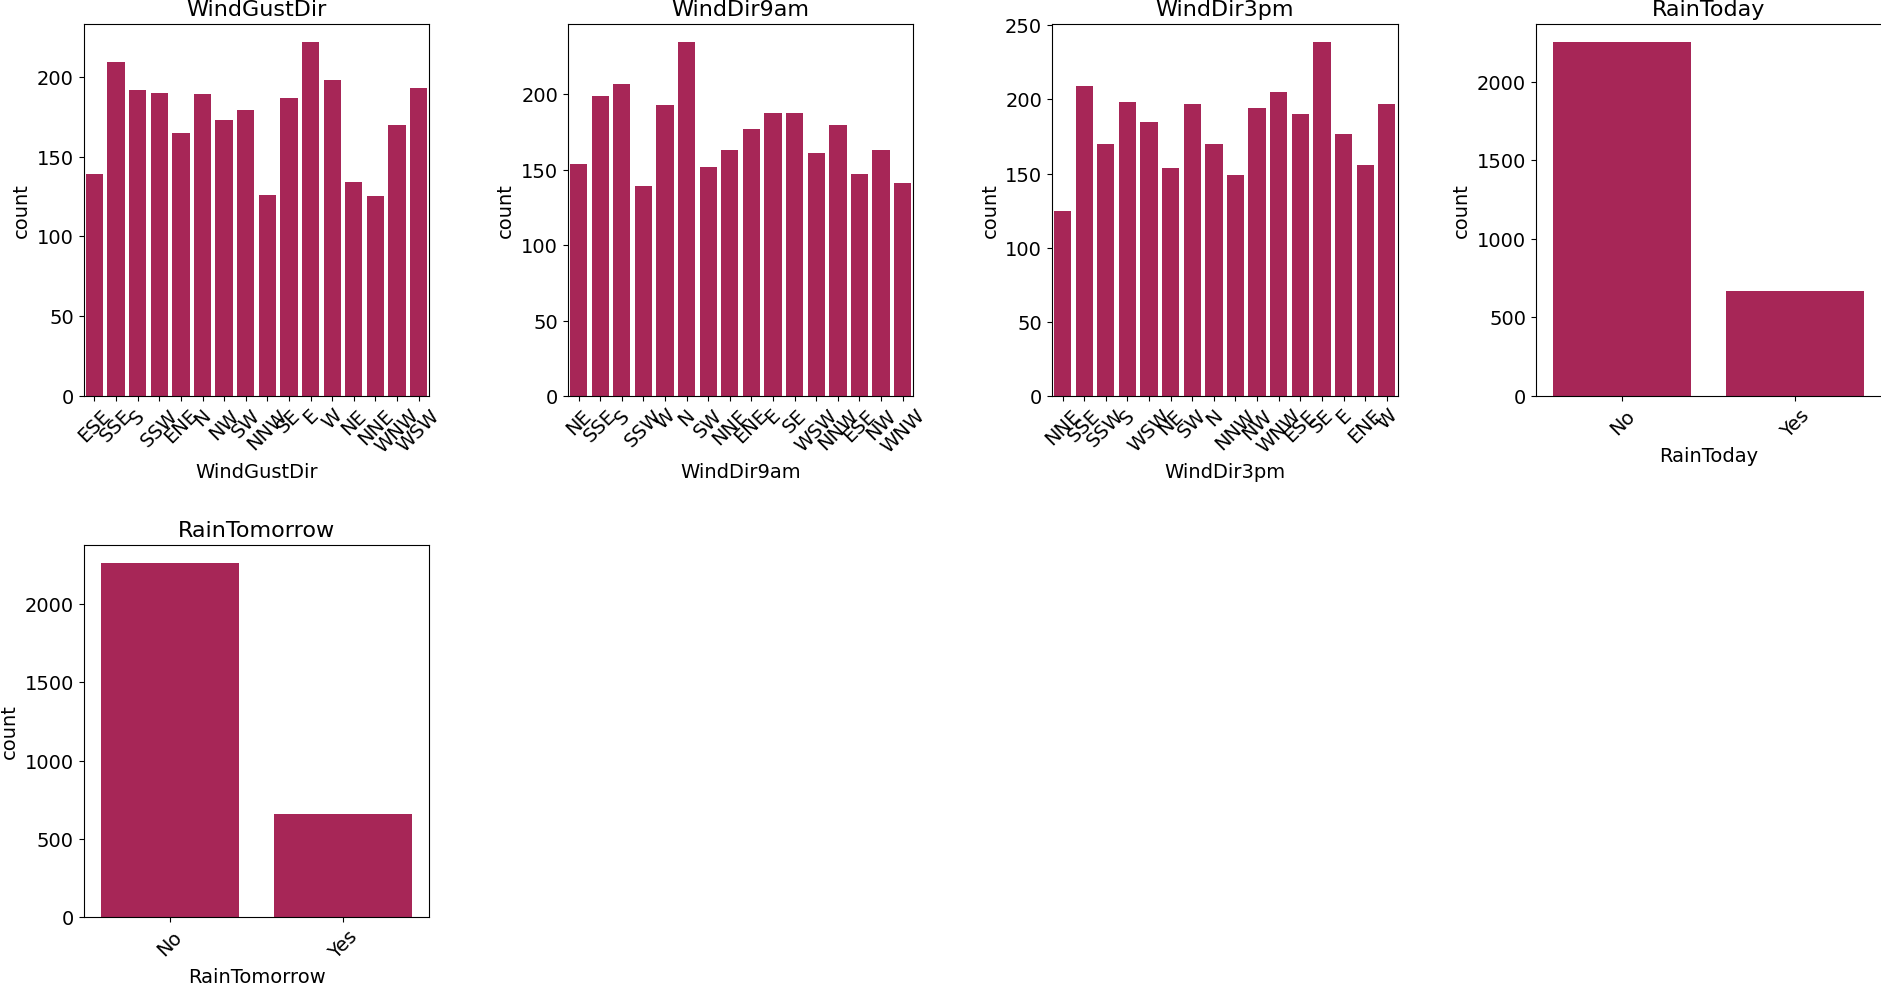
\includegraphics[width=460px]{EDA/bar_charts.png}%
\caption{Bar Charts of Categorical columns}%
\end{figure}

%
\newpage%
\section{Evaluation Metrics}%
\label{sec:EvaluationMetrics}%
\subsection{Accuracy}%
\label{subsec:Accuracy}%

                \textbf{Accuracy} is one of the simplest evaluation metrics for classification models. 
                It is defined as the ratio of correctly predicted observations to the total number of observations:

                \[
                \text{Accuracy} = \frac{\text{Number of Correct Predictions}}{\text{Total Number of Predictions}}
                \]

                While accuracy is intuitive and easy to understand, it may not be suitable for imbalanced datasets. 
                For example, in a dataset where 95\% of the samples belong to one class, predicting the majority class for every instance 
                would result in high accuracy but poor performance on the minority class.
                

%
\subsection{F1 Score}%
\label{subsec:F1Score}%

                The \textbf{F1 Score} is the harmonic mean of Precision and Recall, providing a balance between the two. 
                It is particularly useful when dealing with imbalanced datasets. Precision and Recall are defined as follows:

                \[
                \text{Precision} = \frac{\text{True Positives}}{\text{True Positives} + \text{False Positives}}
                \]
                \[
                \text{Recall} = \frac{\text{True Positives}}{\text{True Positives} + \text{False Negatives}}
                \]

                The F1 Score combines these metrics:

                \[
                \text{F1 Score} = 2 \cdot \frac{\text{Precision} \cdot \text{Recall}}{\text{Precision} + \text{Recall}}
                \]

                A high F1 Score indicates a good balance between Precision and Recall, making it a valuable metric in scenarios where false positives 
                and false negatives have significant costs.
                

%
\subsection{ROC AUC}%
\label{subsec:ROCAUC}%

                The Receiver Operating Characteristic (ROC) curve plots the True Positive Rate (Recall) against the False Positive Rate at various threshold settings. 
                The \textbf{Area Under the Curve (AUC) of the ROC curve} measures the overall ability of the model to distinguish between classes. 

                \[
                \text{AUC} = \int_{\text{FPR}=0}^{1} \text{TPR}(\text{FPR}) \, d(\text{FPR})
                \]

                Key points about ROC AUC:
                \begin{itemize}
                    \item An AUC of 0.5 indicates random guessing.
                    \item An AUC of 1.0 indicates perfect classification.
                    \item It is a threshold-independent metric, providing an aggregate measure of performance across all classification thresholds.
                \end{itemize}

                ROC AUC is particularly useful for binary classification tasks and provides insights into the trade-off between sensitivity and specificity.
                

%
\newpage%
\section{Model Optimization Results}%
\label{sec:ModelOptimizationResults}%
\subsection{Optimization Results Tables}%
\label{subsec:OptimizationResultsTables}%
The tables below show the hyperparameters and achieved metrics for each model configuration considered during the optimization process. The index of models with default hyperparameters is 0. The next models, indexed from 1, were chosen by Random Search.%


\begin{table}[h!]%
\caption{Random Forest Hyperparameters and achivied metrics}%
\vspace{0.2cm}%
\centering%
\begin{tabular}{|c||c||c||c||c||c||c||c||c||c|}%
\hline%
Index&Metric/Hyperp.\textbackslash{} Iteration&0&1&2&3&4&5&6&7\\%
\hline%
0&f1&0.9525&0.7757&0.9295&0.8254&0.9112&0.9203&0.7808&0.8335\\%
1&accuracy&0.9525&0.7757&0.9296&0.8254&0.9113&0.9203&0.7808&0.8338\\%
2&roc\_auc&0.9928&0.865&0.9826&0.9119&0.9718&0.9781&0.8653&0.9028\\%
3&n\_estimators&100&200&50&50&50&200&50&500\\%
4&criterion&gini&entropy&entropy&gini&log\_loss&entropy&entropy&entropy\\%
5&max\_depth&None&30&None&20&30&20&20&10\\%
6&min\_samples\_split&2&5&2&10&2&10&5&5\\%
7&min\_samples\_leaf&1&1&2&1&4&2&4&1\\%
8&min\_weight\_fraction\_leaf&0.0&0.05&0.0&0.01&0.0&0.0&0.05&0.0\\%
9&max\_features&sqrt&sqrt&sqrt&log2&None&sqrt&log2&None\\%
10&bootstrap&1&1&1&0&1&1&1&0\\%
\hline%
\end{tabular}%
\end{table}

%


\begin{table}[h!]%
\caption{Decision Tree Hyperparameters and achivied metrics}%
\vspace{0.2cm}%
\centering%
\begin{tabular}{|c||c||c||c||c||c||c||c||c||c|}%
\hline%
Index&Metric/Hyperp. \textbackslash{} Iteration&0&1&2&3&4&5&6&7\\%
\hline%
0&f1&0.9136&0.8703&0.8717&0.7644&0.6842&0.6842&0.7943&0.6842\\%
1&accuracy&0.9139&0.8706&0.8722&0.7645&0.6987&0.6987&0.7945&0.6987\\%
2&roc\_auc&0.9139&0.8982&0.9003&0.8276&0.6916&0.6916&0.8768&0.6916\\%
3&criterion&gini&entropy&gini&log\_loss&gini&entropy&entropy&entropy\\%
4&splitter&best&random&random&best&random&random&random&random\\%
5&max\_depth&None&30&None&10&10&20&40&10\\%
6&min\_samples\_split&2&5&2&5&10&2&10&5\\%
7&min\_samples\_leaf&1&1&2&4&1&2&4&1\\%
8&max\_features&None&sqrt&None&None&None&None&log2&log2\\%
9&class\_weight&None&balanced&balanced&None&None&None&balanced&None\\%
10&min\_impurity\_decrease&0.0&0.0&0.0&0.01&0.05&0.05&0.0&0.1\\%
\hline%
\end{tabular}%
\end{table}

%


\begin{table}[h!]%
\caption{XGBoost Hyperparameters and achivied metrics}%
\vspace{0.2cm}%
\centering%
\begin{tabular}{|c||c||c||c||c||c||c||c||c||c|}%
\hline%
Index&Metric/Hyperp. \textbackslash{} Iteration&0&1&2&3&4&5&6&7\\%
\hline%
0&f1&0.9437&0.9348&0.8898&0.9206&0.8829&0.9352&0.9286&0.9361\\%
1&accuracy&0.9437&0.9349&0.8898&0.9208&0.883&0.9353&0.9287&0.9362\\%
2&roc\_auc&0.9872&0.9766&0.9555&0.9696&0.9432&0.9815&0.9749&0.9813\\%
3&eval\_metric&logloss&logloss&logloss&logloss&logloss&logloss&logloss&logloss\\%
4&n\_estimators&100&500&50&500&200&500&100&200\\%
5&max\_depth&6&15&10&3&3&10&15&10\\%
6&learning\_rate&0.3&0.1&0.01&0.2&0.2&0.05&0.2&0.1\\%
7&subsample&1.0&0.5&0.9&0.7&0.5&0.9&1.0&0.7\\%
8&colsample\_bytree&1.0&0.9&0.5&0.5&0.5&0.7&0.7&0.7\\%
9&min\_child\_weight&1&5&1&1&5&1&7&1\\%
10&gamma&0.0&0.0&0.1&0.1&0.2&0.1&0.0&0.2\\%
11&reg\_alpha&0.0&0.0&0.1&0.1&1.0&1.0&1.0&0.0\\%
12&reg\_lambda&1.0&5.0&1.5&2.0&2.0&5.0&1.0&5.0\\%
\hline%
\end{tabular}%
\end{table}

%
\newpage%
\subsection{Boxplots of accuracy, f1, roc\_auc}%
\label{subsec:Boxplotsofaccuracy,f1,rocauc}%
Boxplots of accuracy, F1, and ROC AUC illustrate the distribution and variability of model performance metrics across different configurations of hyperparameters. The plots are located below.%


\begin{figure}[h!]%
\centering%
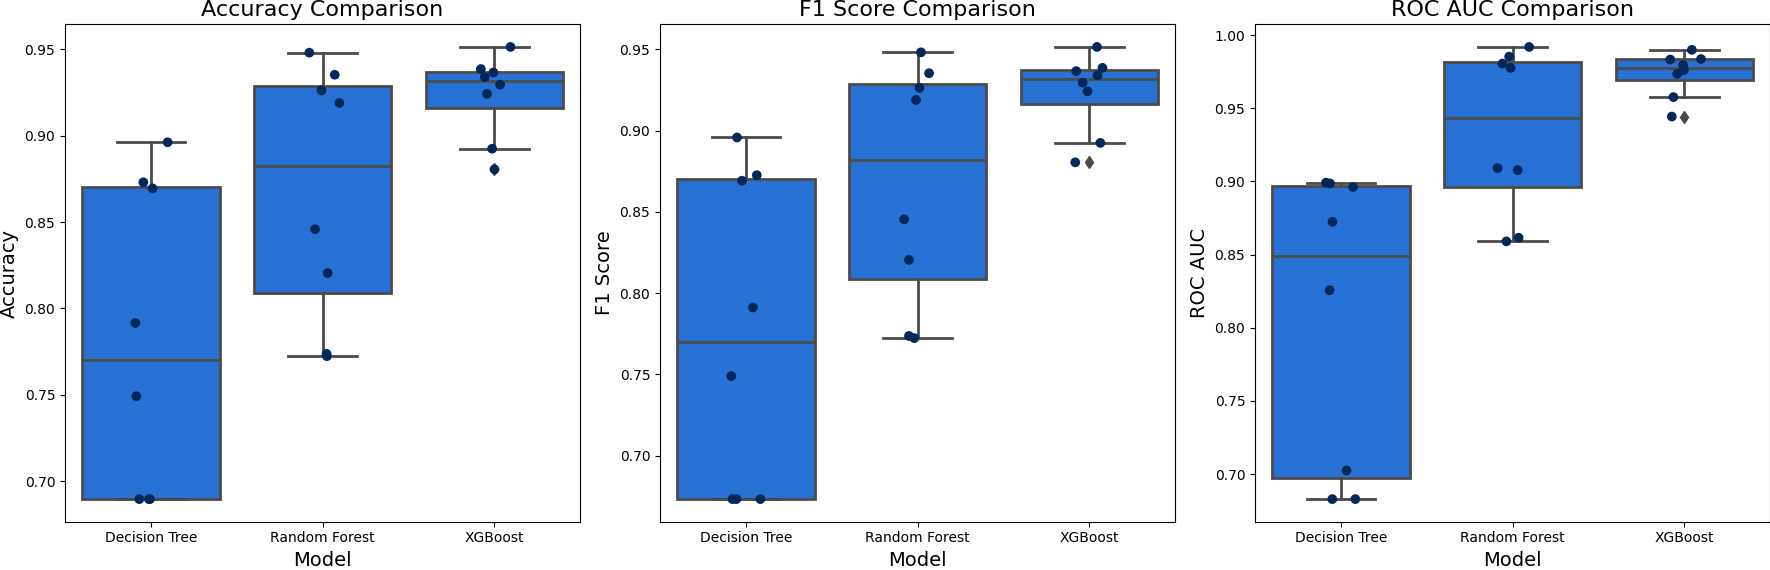
\includegraphics[width=460px]{ModelOptimization/box_plots_metrics.png}%
\caption{Boxplots of accuracy, f1, roc\_auc}%
\end{figure}

%
\subsection{Barplots of maximum values of metrics achievied by model}%
\label{subsec:Barplotsofmaximumvaluesofmetricsachieviedbymodel}%
Barplots of maximum metric values show the highest performance scores for each model type. The plots are located below.%


\begin{figure}[h!]%
\centering%
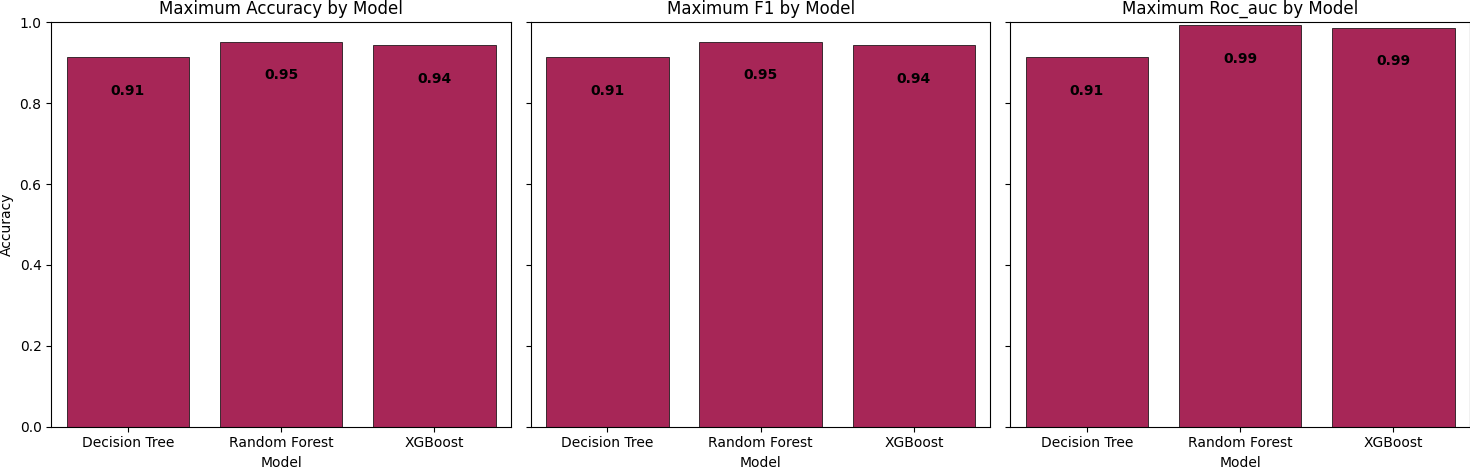
\includegraphics[width=460px]{ModelOptimization/barplots_max_metric.png}%
\caption{Barplots of maximum values of metrics achievied by model}%
\end{figure}

%
\newpage%
\section{Interpretabilty of the best models}%
\label{sec:Interpretabiltyofthebestmodels}%
Classify2TeX package defined the best model as the one that achievied the highest value of a metric, chosen by the user, or ROC AUC by default.%
In this case, the optimization process was aimed at maximizing%
\textbf{ Accuracy.}%
\\%
Do not forget, that after preprocessing, columns names have changed, because of transformations of categorical features.%
\subsection{SHAP {-} what is under the hood?}%
\label{subsec:SHAP{-}whatisunderthehood?}%

        \textbf{SHAP (SHapley Additive exPlanations) values} are a unified measure of feature importance, grounded in cooperative game theory, that explain the contribution of each feature to the predictions of a machine learning model. By assigning a consistent and fair contribution to each feature, SHAP values offer insights into the underlying decision-making process of the model, both for specific predictions and overall feature importance.
        %

        The fundamental principle behind SHAP is that a model’s prediction for a given instance can be decomposed into the sum of contributions from its features, along with a baseline value. The baseline typically represents the average model prediction across the dataset when no feature information is provided.
        %

        \subsection*{How SHAP Values work}
        %

        For a specific instance, SHAP calculates how much each feature contributes to the difference between the baseline and the model's prediction. This involves:
        %

        \begin{enumerate}
            \item \textbf{Marginal Contributions}: Evaluating how the prediction changes when each feature is added to subsets of other features. For example, if you have features \( A, B, C \), SHAP will compute how the prediction changes when \( A \) is added to subsets like \( \{\}, \{ B \}, \{ C \}, \{ B, C \} \), etc.
            \item \textbf{Weighted Averaging Across Subsets}: To compute the SHAP value for a feature, the method takes the average of its marginal contributions across all subsets of features, weighted by the size of the subsets. This ensures fairness in the distribution of contributions.
            \item \textbf{Baseline Value}: The baseline is a reference point, usually the average model prediction over the dataset. It represents what the model predicts when no features are considered.
        \end{enumerate}
        %

        For any given data point, SHAP values indicate how much each feature shifts the model’s prediction relative to the baseline. A positive SHAP value means the feature increases the prediction, while a negative SHAP value means it decreases the prediction. This decomposition allows for a granular understanding of both the direction and magnitude of each feature's influence on the model’s decision.

%
\newpage%
\subsection{The best XGBoost model Explanation}%
\label{subsec:ThebestXGBoostmodelExplanation}%
\subsubsection{XGBoost model {-} feature importance using SHAP values}%
\label{ssubsec:XGBoostmodel{-}featureimportanceusingSHAPvalues}%

        \textbf{SHAP bar plot} provides a concise overview of the importance of individual features in the model's predictions. 
        Each bar represents a feature, with its length corresponding to the mean absolute SHAP value across all samples. 
        This indicates the average magnitude of the feature's contribution to the predictions, regardless of direction.
        %

        \hspace{20px}Features are ranked in descending order of importance, and only the top 15 features are displayed by default for clarity.
        The bar plot allows quick identification of the most influential features driving the model's behavior and is particularly useful for comparing their relative contributions.\\
        \newline                     
        %


\begin{figure}[h!]%
\centering%
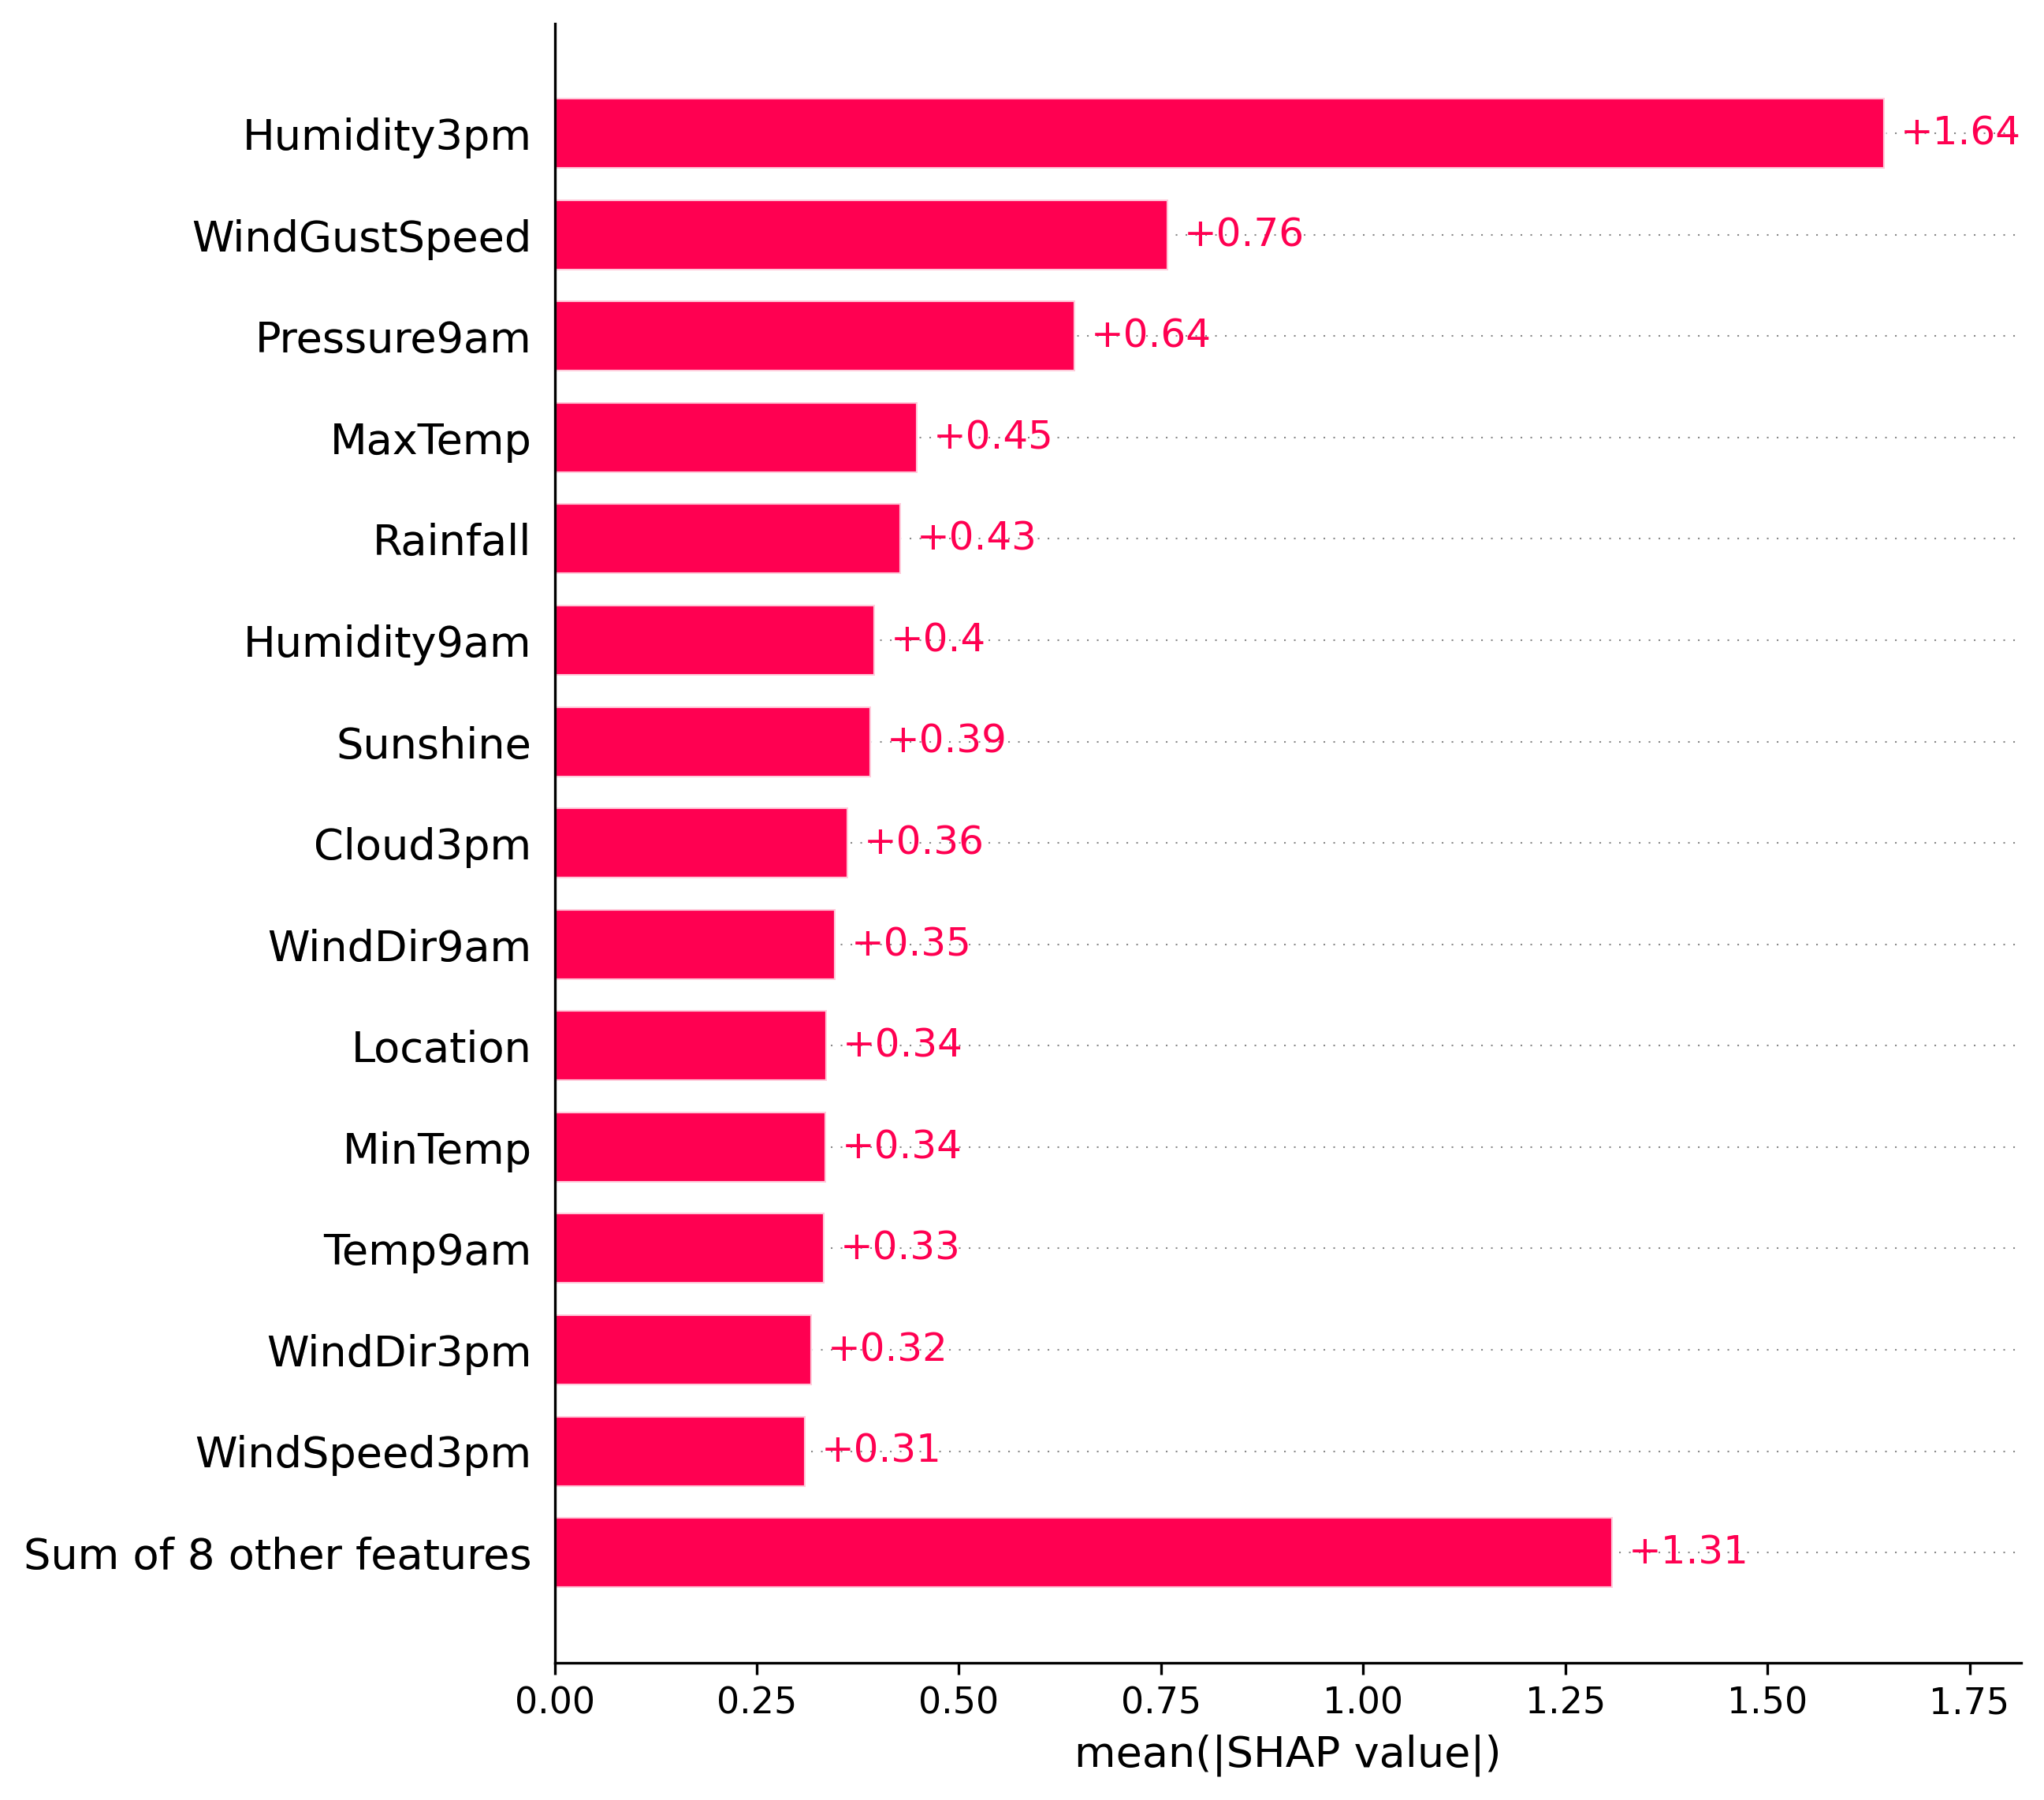
\includegraphics[width=350px]{XAI/XGBoost/global_feature_importance_shap.png}%
\caption{SHAP values for the best XGBoost model}%
\end{figure}

%
\newpage%
\subsubsection{XGBoost model {-} feature importance gained directly from the model}%
\label{ssubsec:XGBoostmodel{-}featureimportancegaineddirectlyfromthemodel}%

        \textbf{Feature importance bar chart:} visually represents the contributions of individual features to the model's predictions, 
        based on their calculated importance scores. Each bar in the chart corresponds to a feature, and its length indicates the magnitude of 
        that feature's importance in reducing split impurity during the model's training process. Features that contribute more significantly to 
        the model's predictive accuracy are displayed with longer bars, while less influential features have shorter bars.
        %

        \hspace{20px}The chart is horizontally oriented, with feature names listed on the vertical axis and their corresponding importance values on the horizontal axis.
        %

        \hspace{20px}This visualization is especially useful for diagnosing the model's behavior, understanding which features drive its decisions, 
        and identifying variables that have the most impact on predictions.\\
        \newline
        %


\begin{figure}[h!]%
\centering%
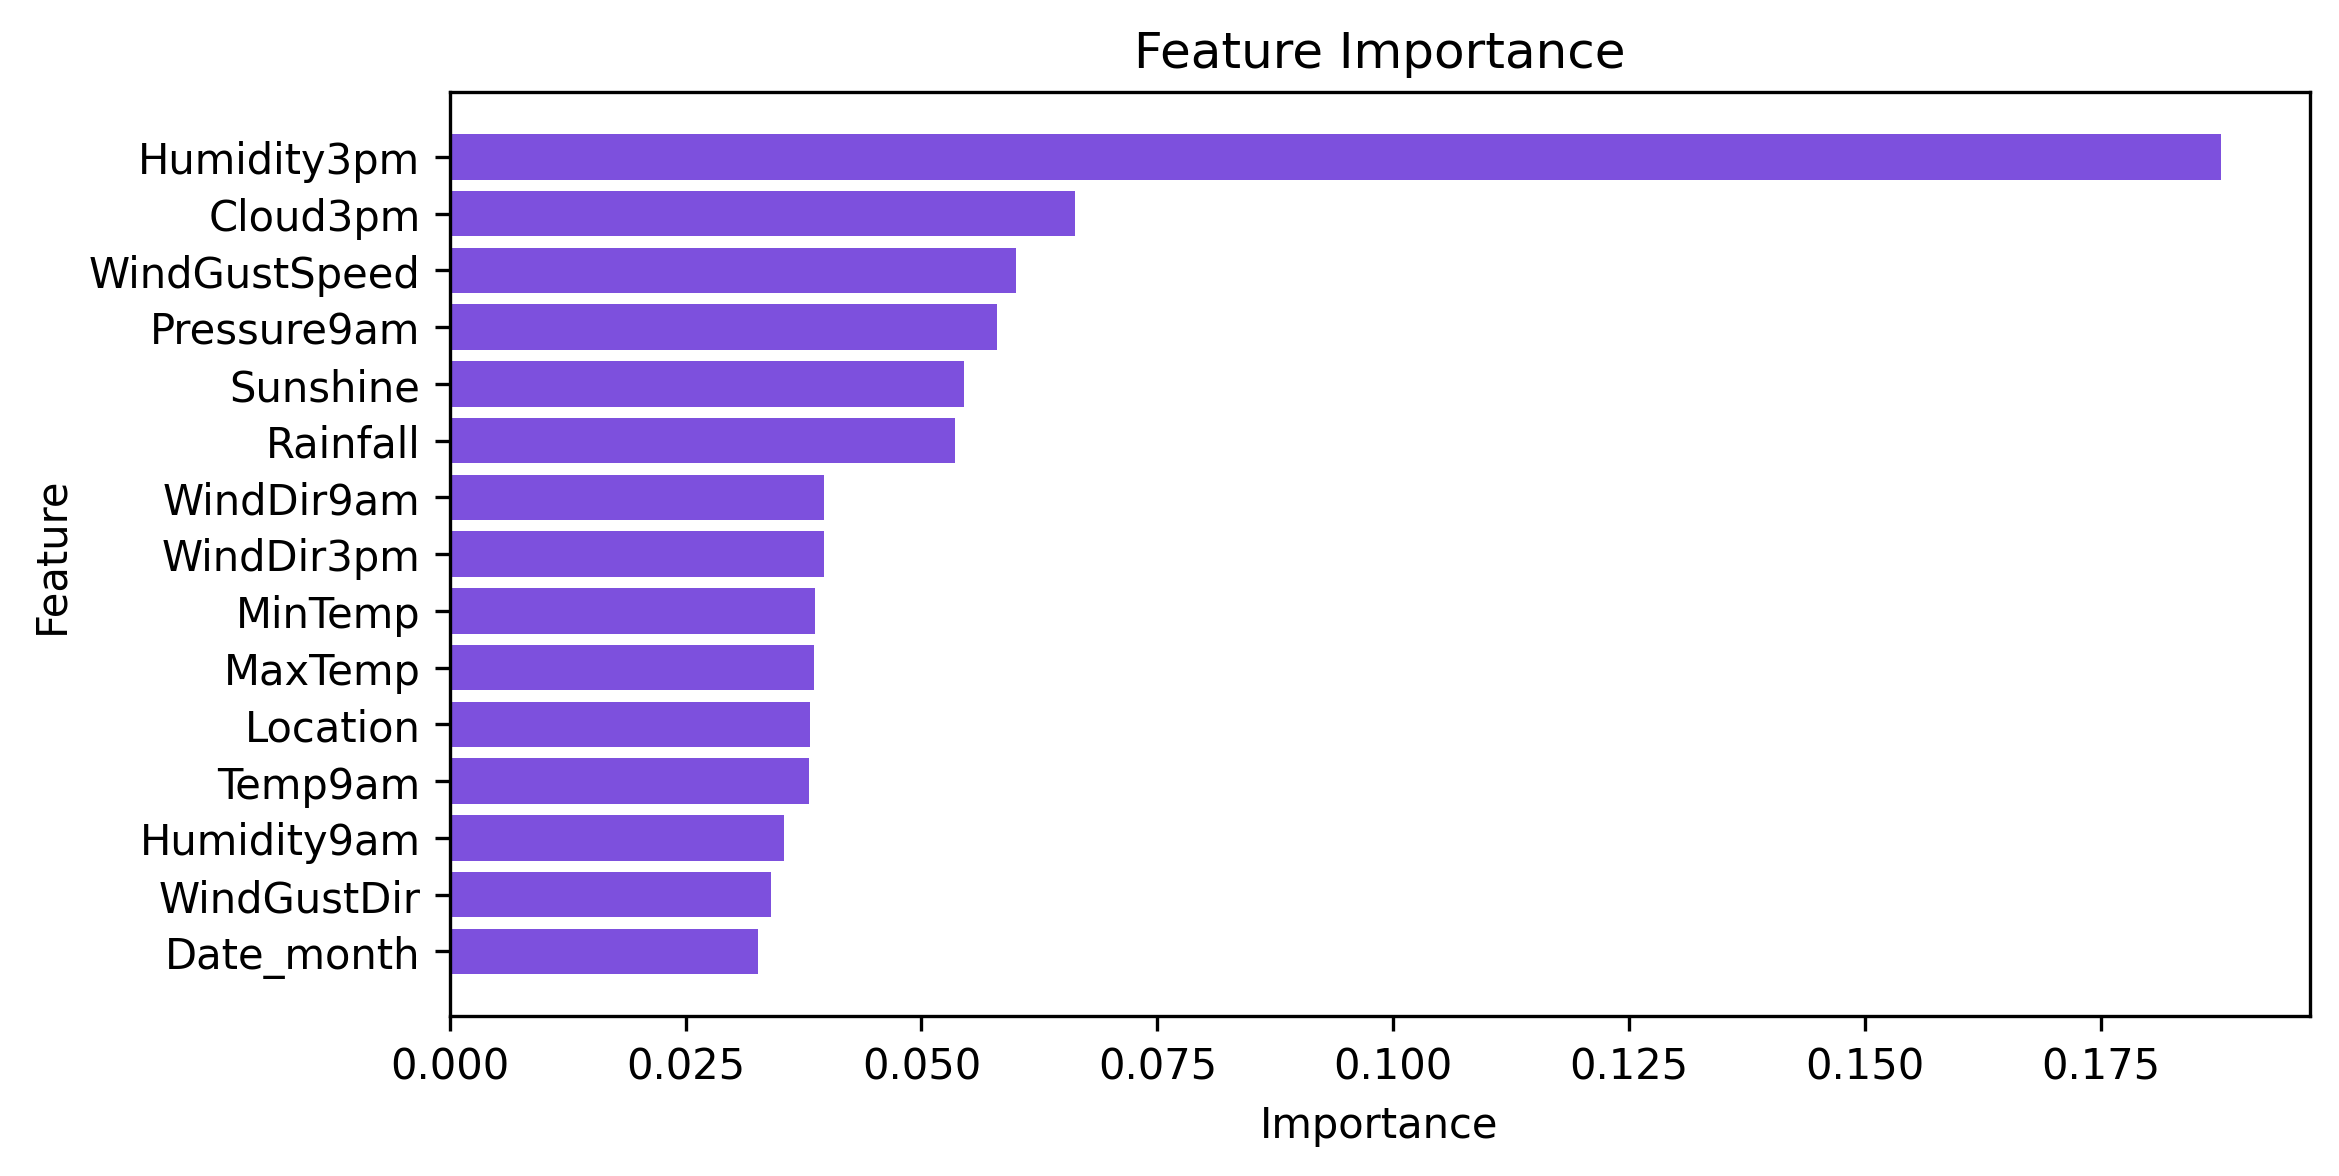
\includegraphics[width=350px]{XAI/XGBoost/feature_importance.png}%
\caption{Feature Importance for the best XGBoost model}%
\end{figure}

%
\newpage%
\subsubsection{XGBoost model {-} violin plot (SHAP) of impact on prediction}%
\label{ssubsec:XGBoostmodel{-}violinplot(SHAP)ofimpactonprediction}%

        \textbf{SHAP violin plot} provides a visual summary of how each feature influences model predictions and the variability of this influence. 
        Features are listed on the vertical axis in descending order of importance, while the horizontal axis shows SHAP values, 
        indicating the magnitude and direction of each feature's contribution to predictions.
        %

        \hspace{20px}The shape of each 'violin' represents the distribution of SHAP values for a feature: wider sections indicate higher density of similar values, 
        while narrower sections show less frequent SHAP values. Positive SHAP values increase the prediction, and negative values decrease it.
        %

        \hspace{20px} Colors correspond to actual feature values, with red typically representing higher values and blue lower ones.
        The color distribution along the SHAP scale highlights how feature values affect predictions; for instance, 
        if red dominates the positive side, high feature values increase predictions.
        %

        \hspace{10px} By default, only the top 15 features by importance are displayed, keeping the visualization focused and interpretable.\\
        %


\begin{figure}[h!]%
\centering%
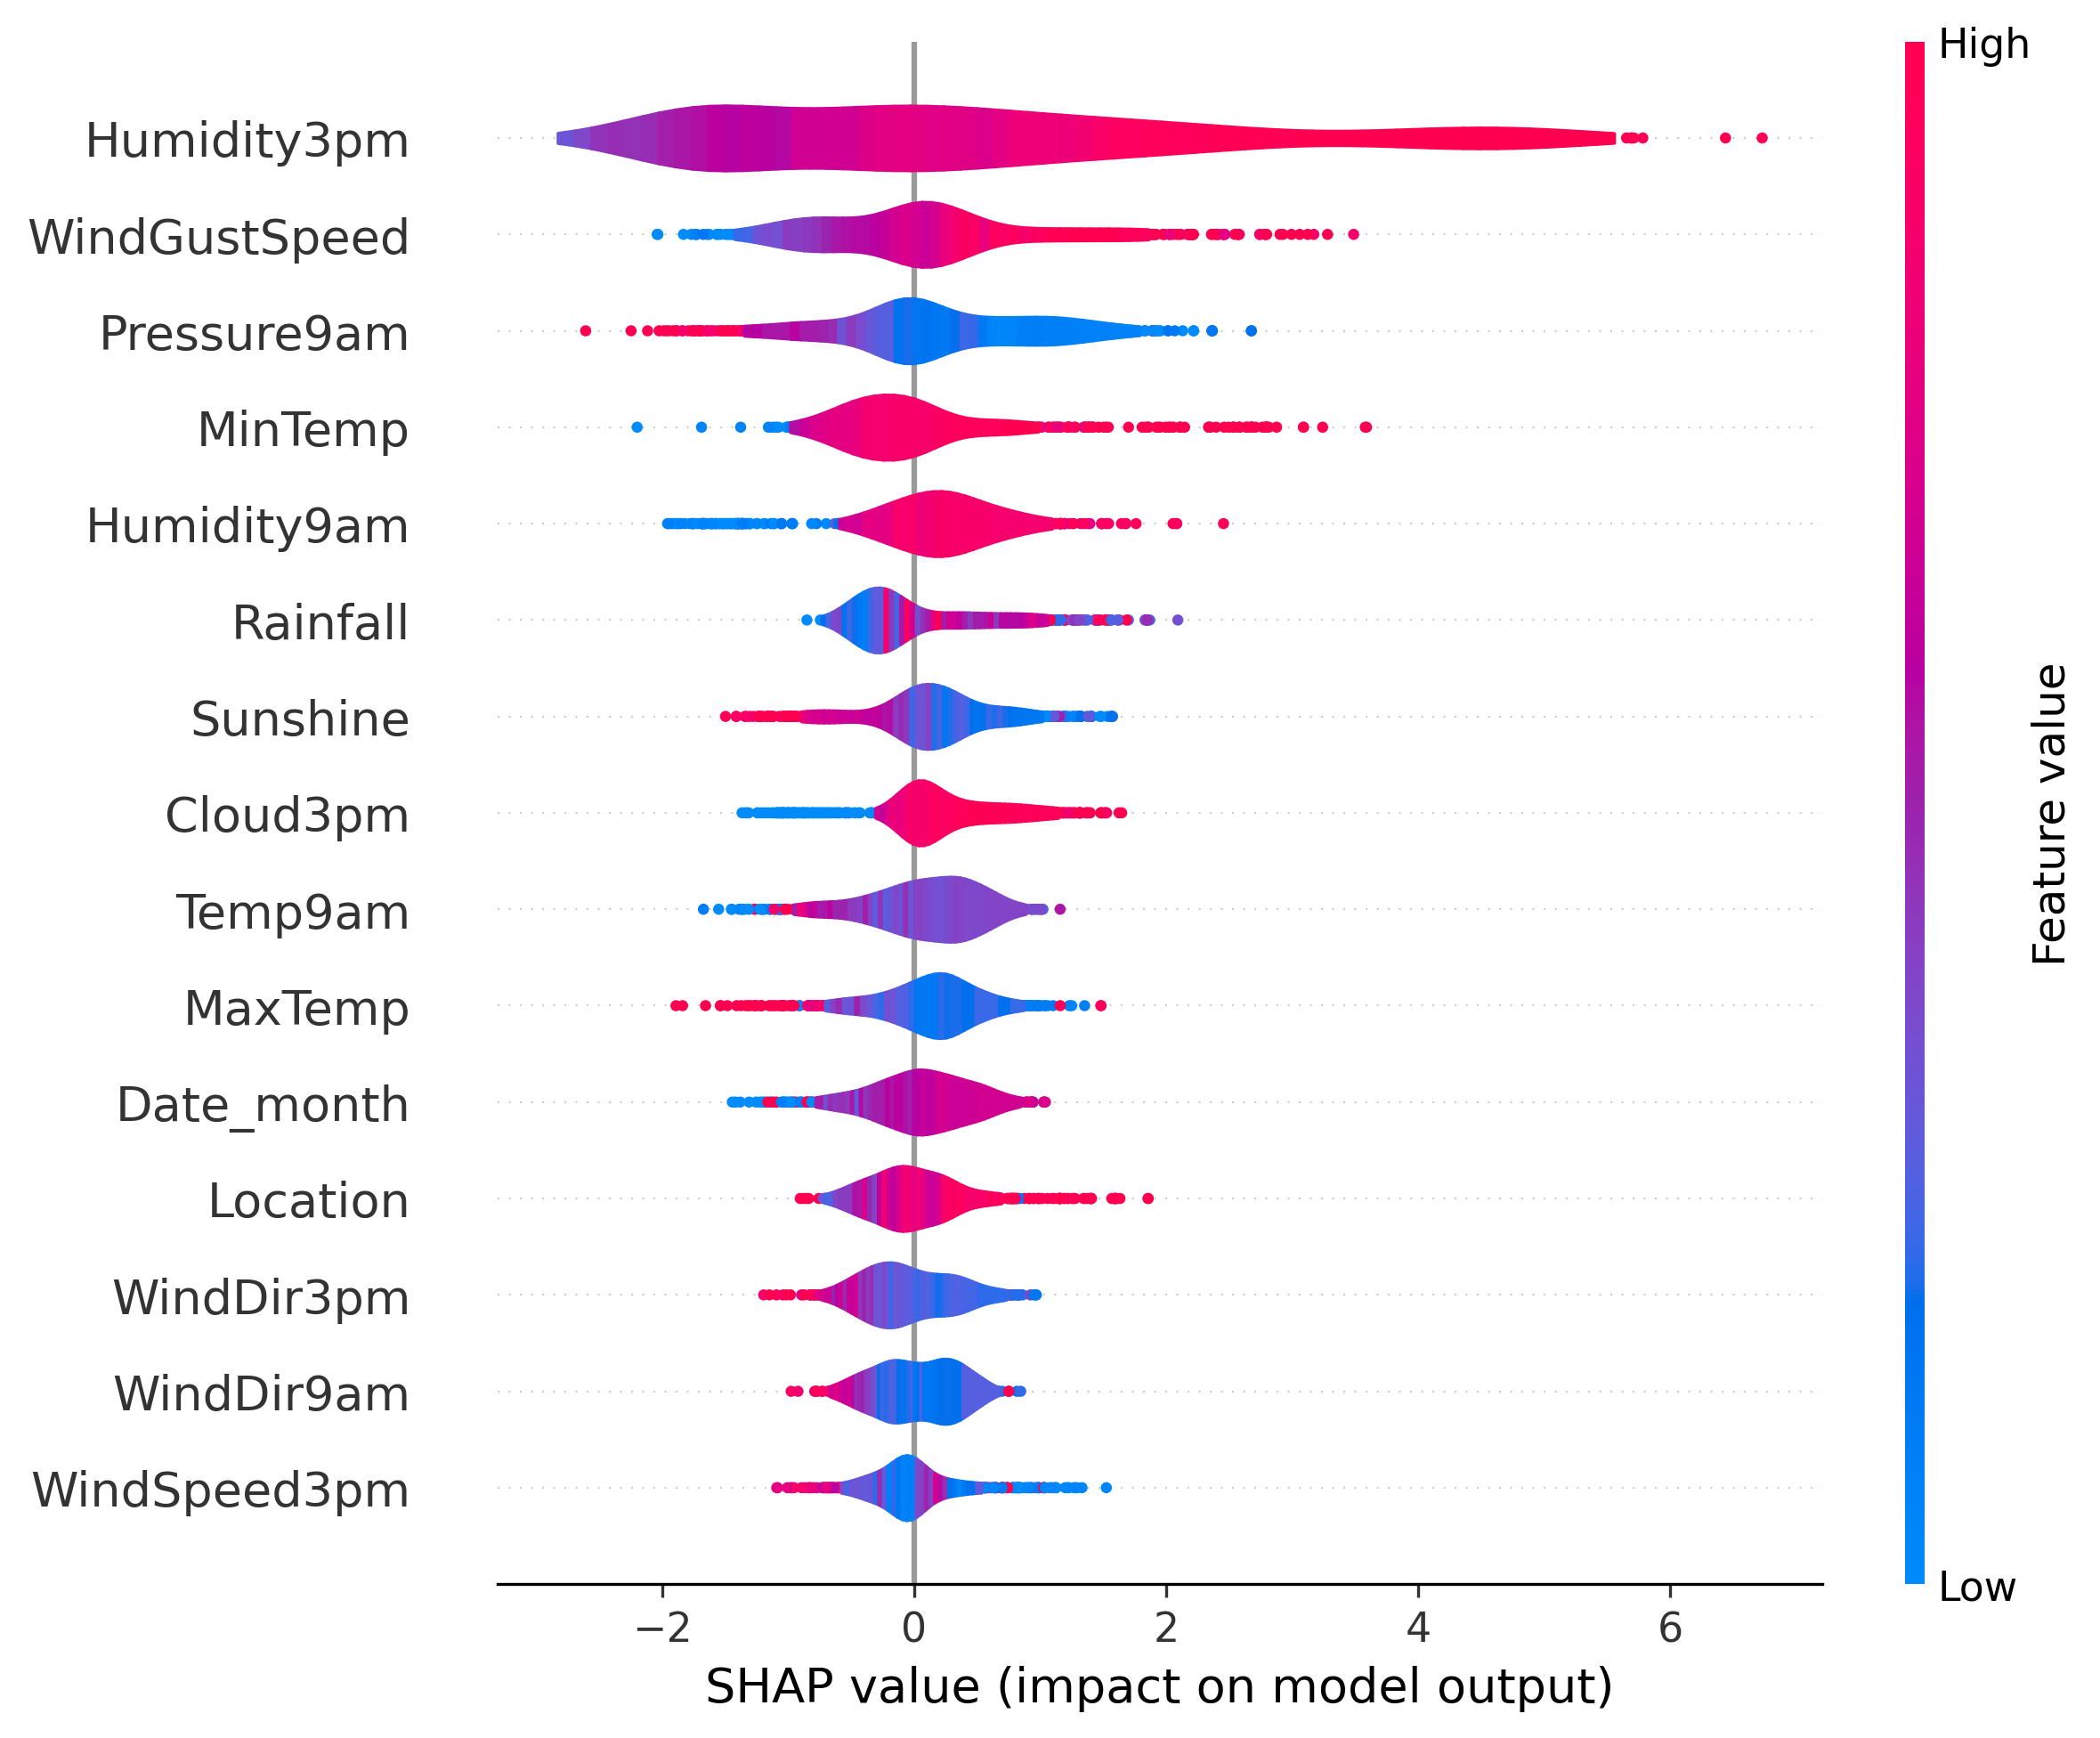
\includegraphics[width=400px]{XAI/XGBoost/violin_summary_plot_shap.png}%
\caption{Violin plot (SHAP) of impact on prediction for the best default XGBoost model}%
\end{figure}

%
\end{document}